\documentclass[norsk,a4paper,12pt]{article}
\usepackage[T1]{fontenc} %for å bruke æøå
\usepackage[utf8]{inputenc}
\usepackage{graphicx} %for å inkludere grafikk
\usepackage{verbatim} %for å inkludere filer med tegn LaTeX ikke liker
\usepackage{amsfonts}
%\usepackage[framed]{mcode} %for å få inn matlabkode
\usepackage{listings}
\usepackage[margin=1.2cm]{caption} % skalere figur text
\usepackage{subfigure}

\bibliographystyle{plain}
\usepackage{parskip}
\usepackage{babel, textcomp, color, amsmath, amssymb, tikz, subfig, float}
\renewcommand{\captionfont}{\sffamily\small} 
\renewcommand{\captionlabelfont}{\bf} 
\fboxsep=0mm % ramme inn bilder


\title{FYS3150 - Project 2}
\author{Steffen Brask}
\date{\today}


\begin{document}

\maketitle

%\begin{center}
%Skrive noe smart her? GIT link?
%\end{center}


\newpage


\section*{Abstract}

This is a study on solving the schrödinger equation numerically with the jacobi rotation algorithm.
It addresses problems based on the setup of the algorithm, and takes a look at solutions for quantum systems
which are confined to a small space, or so-called quantum dots.

\section*{Introduction}

We will in this project mainly address two problems. How to solve the schrödinger equation numerically. and what happens when we
confine the quantum system to a small space.

Solving the schrödinger equation (or SE) can be very hard or fairly easy. In this project we will be in between those two.
We will take some ''shortcuts'' like assuming that the quantum number l is equal to zero. But this is fine in this project because
the goal is to see what happens in the spatial dimensions because this is directly related to various properties of quantum dots.


\section*{Solution}

\subsection*{Rewriting the Schrödinger equation}

Our first task will be to rewrite the schrödinger equation to a more ''programmable'' form.
We can start with the general 3 dimensional SE:

\begin{equation}
 -\frac{\hbar^2}{2m}\nabla^2\psi(\vec{r}) + V(\vec{r})\psi(\vec{r}) = E\psi(\vec{r})
\end{equation}

For this project we are only interested in the radial part of the schrödinger equation.
And for one electron this equation can be written: 

\begin{equation}
 -\frac{\hbar^2}{2 m} \left ( \frac{1}{r^2} \frac{d}{dr} r^2
  \frac{d}{dr} - \frac{l (l + 1)}{r^2} \right )R(r) 
     + V(r) R(r) = E R(r).
\end{equation}

This equation is transformed to spherical coordinates, and in we use the harmonic oscillator potential for $V(r) = \frac{1}{2}kr^2$ with $k = m\omega^2$.
We have now assumed spherical symmetry, and for simplicity we assume that there is no orbital momentum so $l = 0$
The energies in three dimensions can then be written

\begin{equation}
 E_{n}=  \hbar \omega \left(2n+\frac{3}{2}\right)
\end{equation}

% With N = 0,1,2... We now substitute $R(r) = \frac{1}{r}u(r)$, and introduce the dimensionless variable $\rho(r) = \frac{1}{\alpha}r$
so that we end up with:

\begin{equation}
 -\frac{\hbar^2}{2 m \alpha^2} \frac{d^2}{d\rho^2} u(\rho) 
       + \frac{k}{2} \alpha^2\rho^2u(\rho)  = E u(\rho) 
\end{equation}

or multiplying with $2m\alpha^2/\hbar^2$:

\begin{equation}
 -\frac{d^2}{d\rho^2} u(\rho) 
       + \frac{mk}{\hbar^2} \alpha^4\rho^2u(\rho)  = \frac{2m\alpha^2}{\hbar^2}E u(\rho) .
\end{equation}

for the sake of simplicity (or numerical precision), we fix $\frac{mk}{\hbar^2}\alpha^4 = 1$ so that

\begin{equation}
 \alpha = \left(\frac{\hbar^2}{mk}\right)^{1/4}.
\end{equation}

We now define a new variable 

\begin{equation}
 \lambda(E_{n}) = \frac{2m\alpha^2}{\hbar^2}E_{n}
\end{equation}

Later we wil solve the SE for $\lambda$ and we se that with $\lambda$ and $\alpha$ we can find the energy eigenstates $E_{n}$.

The final form we will use to solve numerically is now:

\begin{equation}
 -\frac{d^2}{d\rho^2} u(\rho) + \rho^2u(\rho)  = \lambda u(\rho)
\end{equation}

With boundary conditions $u(0)=0$ and $u(\infty)=0$.


\subsection*{Numerical algorithm}

We will use a similar method as in project 1 for solving this equation. First we rewrite the second derivative of u
to the known form:

\begin{equation}
 u''=\frac{u(\rho+h) -2u(\rho) +u(\rho-h)}{h^2} +O(h^2)
\end{equation}

this form we can use for discrete values of $\rho$ and a step $h$. As usual $h = (\rho_{max} - \rho_{min})/n$, now, in theory 
$\rho_{min} = 0$ and $\rho_{max} = \infty$, but we can not program infinity, we therefore need to chose a $\rho_{max}$ that is ''large enough''
so that $u(\rho_{max}) \simeq 0$. The discrete value of $\rho$ is then $\rho_i = \rho_{min} + ih$. And $u(\rho) = u(\rho_i) = u_i$

we now let:

\begin{equation}
 d_i = \frac{2}{\hbar^2} + V_i, where V_i = \rho_i^2 is the HO potential
\end{equation}

And let:

\begin{equation}
 e_i = -\frac{1}{\hbar^2}
\end{equation}

In this case $e_i$ is a constant, but in general it does not have to. With these definitions we can write the SE on a discrete form:

\begin{equation}
 d_iu_i+e_{i-1}u_{i-1}+e_{i+1}u_{i+1}  = \lambda u_i
\end{equation}

Or as a matrix eigenvalue problem:

\begin{equation}
    \left( \begin{array}{ccccccc} d_1 & e_1 & 0   & 0    & \dots  &0     & 0 \\
                                e_1 & d_2 & e_2 & 0    & \dots  &0     &0 \\
                                0   & e_2 & d_3 & e_3  &0       &\dots & 0\\
                                \dots  & \dots & \dots & \dots  &\dots      &\dots & \dots\\
                                0   & \dots & \dots & \dots  &\dots       &d_{n-1} & e_{n}\\
                                0   & \dots & \dots & \dots  &\dots       &e_{n} & d_{n}

             \end{array} \right)      \left( \begin{array}{c} u_{1} \\
                                                              u_{2} \\
                                                              \dots\\ \dots\\ \dots\\
                                                              u_{n}
             \end{array} \right)=\lambda \left( \begin{array}{c} u_{1} \\
                                                              u_{2} \\
                                                              \dots\\ \dots\\ \dots\\
                                                              u_{n}
             \end{array} \right) 
\end{equation} 

We now implement jacobi's rotation algorithm to solve eq. (13). The trick is to set up a similarity transformation
and minimize the problem until we are left wit a matrix with all diagonal entries being eigenvalues and the rest is zero.

If we let:
\begin{equation}
    {\bf S} = \left(\begin{array}{cccccc}
                           1& 0& \dots & &\dots  &0 \\
                           0 & \dots &  & & &\dots  \\
                           \dots& &cos\theta &\dots &  & sin\theta  \\
                           &   & \dots &1   &\dots & \\
                           &   & \dots &  &\\
                           0&\dots   &-sin\theta  &\dots & &cos\theta \\
                      \end{array} \right)
\end{equation}

A similarity transformation $\bf B = \bf{S^T}\bf{A}\bf{S}$, where A is the SE matrix from above, will perform a plane rotation around
an angle $\theta$. So if we can perform a rotation that minimizes the non diagonal entries (makes them zero) enough times until  
the matrix is in fact a diagonal matrix we will have a solution to our problem. So we chose $\theta$ so that $sin\theta = 0$

This gives us a set of equations to solve numerically, but we first have to define $cot(2\tau) = \tau = (a_{ll} - a_{kk})/2a_{kl}$ where 
$a_{ll}$ and $a_{kk}$ indicates the entries we are rotating about. And then $t = -\tau\pm\sqrt{1+\tau^2}, c = 1/\sqrt{1+t^2}, and s = tc$  
where t stands for tangent, c for cosine, and s for sine.


\begin{lstlisting}[frame=single]
 FindMaxValue(A, max_a, k, l);
 while(max_a < epsilon){
      tau = (a(l,l) - a(k,k))/(2*a(k,l));
	  if( tau > 0 ) {
	      t = 1.0/(tau + sqrt(1.0 + tau*tau));
	  }else{
	      t = -1.0/( -tau + sqrt(1.0 + tau*tau));
	  }
  
	  c = 1/sqrt(1 + t*t);
	  s = t*c;

	  for(int i = 0 ; i < n ; i++) {
	      if(i != k){
		  if(i != l){
		      b(i,k) = a(i,k)*c - a(i,l)*s;
		      b(i,l) = a(i,l)*c + a(i,k)*s;
		      b(k,i) = a(i,k)*c - a(i,l)*s;
		      b(l,i) = a(i,l)*c + a(i,k)*s;
		   }
	      }
	  }
	  b(k,k) = a(k,k)*c*c - 2*a(k,l)*c*s + a(l,l)*s*s;
	  b(l,l) = a(l,l)*c*c + 2*a(k,l)*c*s + a(k,k)*s*s;
	  b(k,l) = 0;
	  b(l,k) = 0;
	  
	  //compute eigenvectors
          for(int i = 0 ; i < n ; i++) {
            r_ik = R(i, k);
            r_il = R(i, l);
            R(i, k) = c*r_ik - s*r_il;
            R(i, l) = c*r_il + s*r_ik;
        }
\end{lstlisting}

This code rotates and minimizes all non-diagonal elements until they are all less than a given epsilon. Here $k$, and $l$
are the indices of the largest entry in a at a given iteration.

We can also find the eigenvectors of the initial matrix $\bf A$ with the last part of code. What we now wish to do is pick out the 
eigenvectors for the the lowest eigenvalues. These will contain the information of the eigenfunctions $\psi$ for the three lowest energy
states of the electron. lets see why this is true:

$\bf A v_i = \lambda_i v_i$

$\bf{S^T}\bf A v_i = \bf{S^T}\lambda_i v_i$

$\bf{S^T}\bf\bf{S}\bf{S^T} A v_i = \bf{S^T}\lambda_i v_i$

since $\bf{S}\bf{S^T} = \bf{I_n}$

so : $\bf{B}\bf{S^T} v_i = \lambda_i \bf{S^T}v_i$ 

we know that the vectors should be orthogonal, so we start with the identity matrix and perform the same rotations on it
witch should give us the eigenvectors. Further we know that the eigenvectors should contain information on the eigenfunctions
since $\lambda$ contains information on the energy $E_n$ so what we end up with is $\hat{\bf{H}}\psi_n = E_n\psi_n$


\section*{Results}

\subsection*{Numerical error}

The first thing we need to do is define n and $\rho$ so that we have an acceptable precision. our choice of n gives us good or 
bad precision for obvious reasons. However, this algorithm is not very effective, it is more a ''brute force'' algorithm.
we should therefore be careful of how large n we use. So what we end up doing is finding a value for $\rho_{max}$ witch is such 
that $u(\rho_{max}) \simeq 0$ this will vary for different energy states, but for the three lowest i found out that 5-6 
gives pretty good precision in our dimensionless case. I found that n = 192 gave me the three lowest eigenvalues with four leading
digits. I could have optimized this further by tinkering with $\rho_{max}$. The algorithm was checked against the Armadillo function for solving eigenvalue problems 

\begin{figure}[H]
  \begin{center}
    \subfigure[]{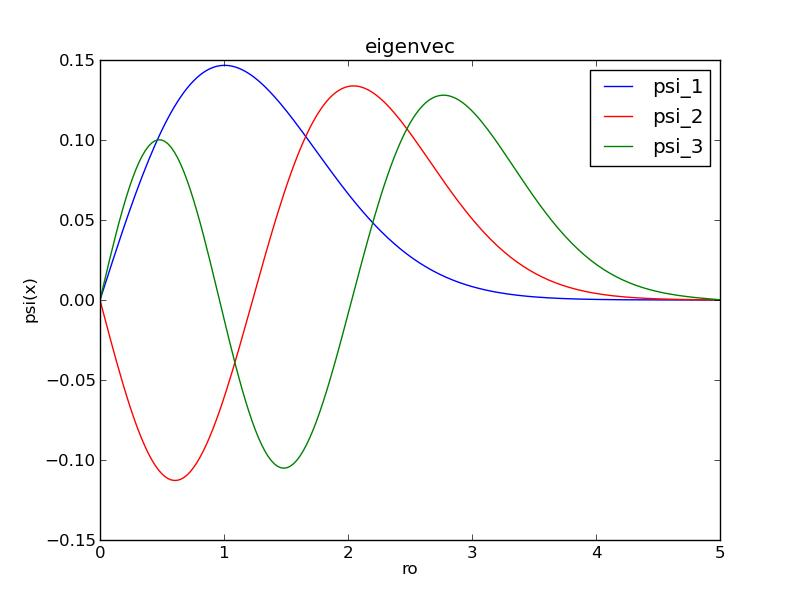
\includegraphics[scale=0.5]{plot_eigenvec.jpg}}
  \end{center}
 \caption{\textit{plot of the three lowest exited states for one electron}}
  \label{fig:edge}
\end{figure}


\subsection*{Quantum dot solution}

We will now study the case for two electrons. We can derive the equation again but the steps are similar to what we did for one electron.
the new equation reads:
\begin{equation}
 -\frac{d^2}{d\rho^2} \psi(\rho) + \omega_r^2\rho^2\psi(\rho) +\frac{1}{\rho} = \lambda \psi(\rho)
\end{equation}

with: $\omega_r^2=\frac{1}{4}\frac{mk}{\hbar^2} \alpha^4, \alpha = \frac{\hbar^2}{m\beta e^2}, \lambda = \frac{m\alpha^2}{\hbar^2}E$.
So the only thing we need to change here is the potential. When the program is run we can clearly see that when we increase $\omega$
we get higher values for $\lambda$ this means that the system has higher values for the energy. $\omega$ reflects the strength
of the oscillator potential, so what we see in table 1 is that with increased $\omega$ the system has higher energy states.

\begin{lstlisting}[frame=single]
 omega = 0,01       0.7290
		    1.8432
		    3.5565

 omega = 0,5        2.2302
		    4.1405
		    6.1676

omega = 1	    4.0576
		    7.9085
		    11.816

omega = 5 	    17.4420
		    37.0405
		    56.7776

\end{lstlisting}
$table 1$

Lets now see how the wave functions for the different values of $\omega$ take form. This is a plot of the eigenvectors against
$\rho_i$.

\begin{figure}[H]
  \begin{center}
    \subfigure[$\omega= 0,01$ ]{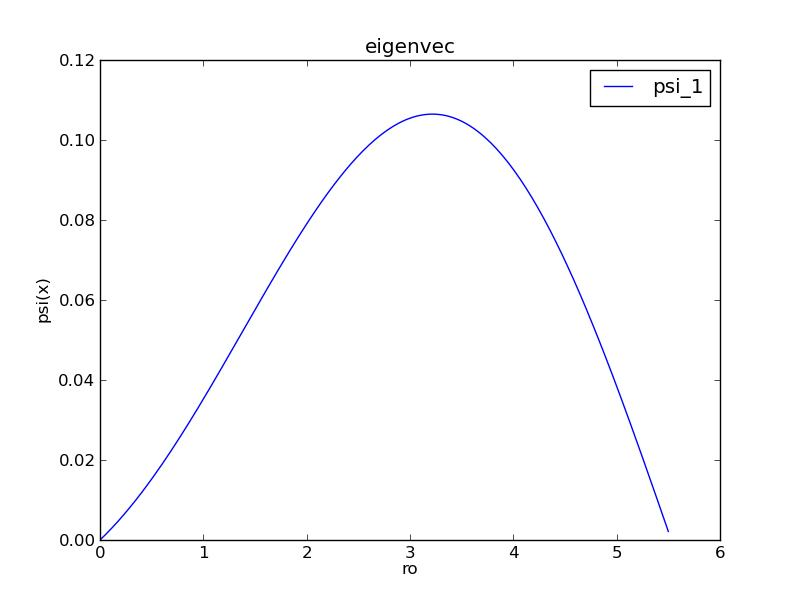
\includegraphics[scale=0.2]{plot_omega_0,01.jpg}}
    \subfigure[$\omega= 0,5$]{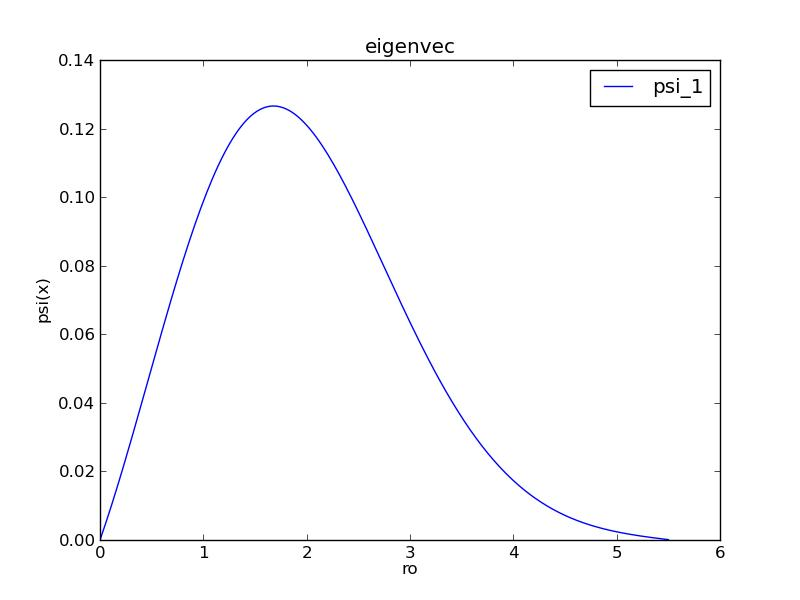
\includegraphics[scale=0.2]{plot_omega_0,5.jpg}}
    \subfigure[$\omega= 1$]{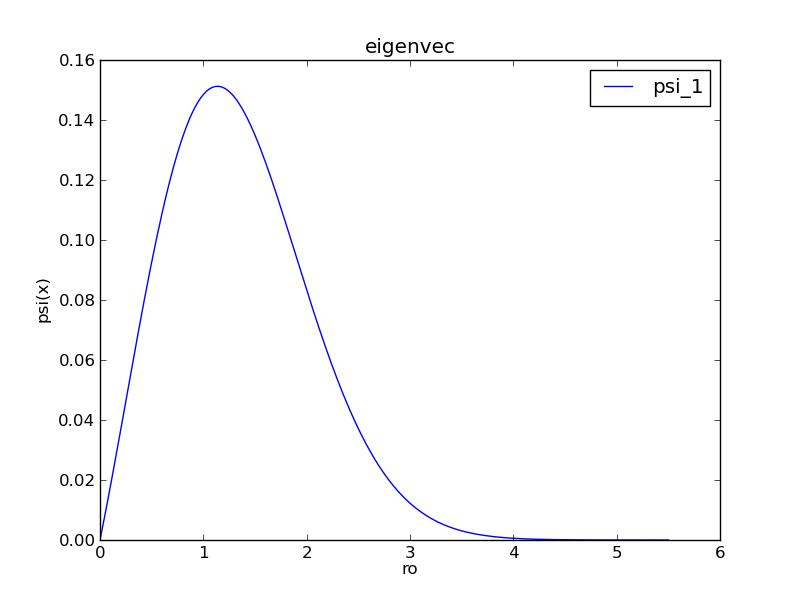
\includegraphics[scale=0.2]{plot_omega_1.jpg}}
    \subfigure[$\omega= 5$]{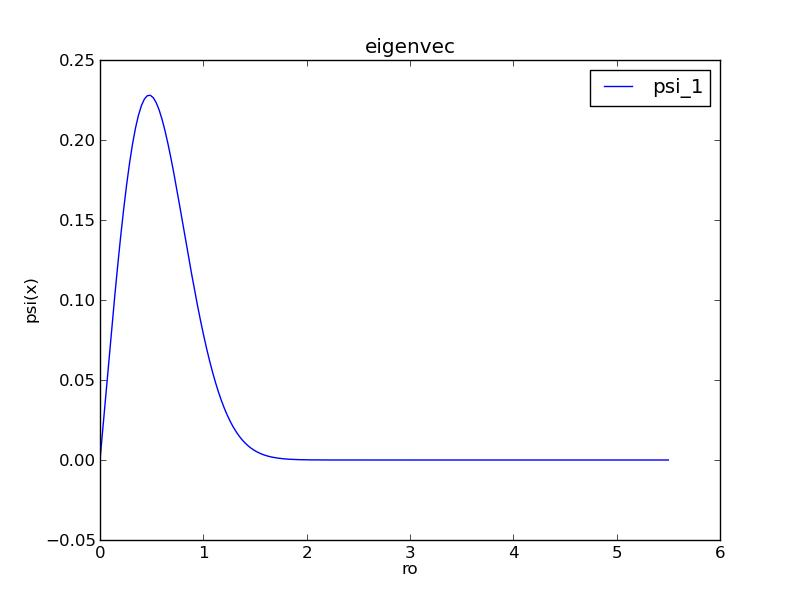
\includegraphics[scale=0.2]{plot_omega_5.jpg}}
  \end{center}
 \caption{\textit{plot of the lowest exited state for two electron problem for different frequency values}}
  \label{fig:edge}
\end{figure}

We see here that the wave function takes different form for the different values of $\omega$. It seems as if the wave function gets
sharper for a higher $\omega$. This can be interpreted like we get a sharper defined position for the electrons relative to each other.
We also see that the highest probability of the position differs for different frequencies. That is, for different potentials.
which means that the relative distance between the electrons gets more fixed and is determined by the potential.


\section*{Conclusion}

What we have done in this project is solve the schrödinger equation numerically by applying the jacobi rotation algorithm.
We then rewrote the equation to apply two electrons. We then solved the equation numerically. What we have found is that when we
place two electrons in a harmonic oscillator well, or a so called ''quantum dot'' we can adjust the systems properties like the radial extension by 
adjusting the potential. (at least we can numerically). 

What does this mean? controlling a quantum system in this way has a huge industrial value. according to wikipedia ''Researchers have studied applications for quantum dots in transistors, solar cells, LEDs, and diode lasers. They have also investigated quantum dots as agents for medical imaging and as possible qubits in quantum computing.''
There is already methods of making quantum dots for different purposes, so this is not a hypothetical result that will never be applied in science.

%\subsection*{}

%\begin{figure}[H]
%  \begin{center}
%    \subfigure[N = 10]{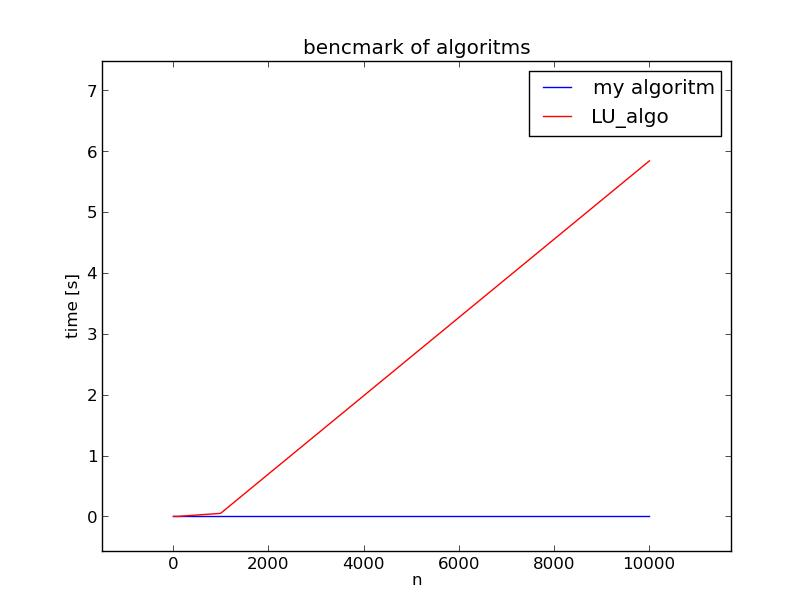
\includegraphics[scale=0.5]{benchmark.jpg}}
%  \end{center}
% \caption{\textit{plot benchmark times for the two different methods of solving}}
%  \label{fig:edge}
%\end{figure}

 
%\newpage

%\section*{Attachments}

%\textbf{Attachment 1: C++ main program}\newline

%\lstinputlisting[language=C++]{main.cpp}

%\newpage

\end{document}








